\documentclass[10pt,letterpaper]{article}
\usepackage[top=0.85in,left=2.75in,footskip=0.75in]{geometry}

% Use adjustwidth environment to exceed column width (see example table in text)
\usepackage{changepage}

% Use Unicode characters when possible
\usepackage[utf8]{inputenc}

% textcomp package and marvosym package for additional characters
\usepackage{textcomp,marvosym}

% fixltx2e package for \textsubscript
\usepackage{fixltx2e}

% amsmath and amssymb packages, useful for mathematical formulas and symbols
\usepackage{amsmath,amssymb}

% cite package, to clean up citations in the main text. Do not remove.
\usepackage{cite}

% Use nameref to cite supporting information files (see Supporting Information section for more info)
\usepackage{nameref,hyperref}

% line numbers
\usepackage[right]{lineno}

% ligatures disabled
\usepackage{microtype}
\DisableLigatures[f]{encoding = *, family = * }

% rotating package for sideways tables
\usepackage{rotating}

% Remove comment for double spacing
\usepackage{setspace} 
\doublespacing

% Text layout
\raggedright
\setlength{\parindent}{0.5cm}
\textwidth 5.25in 
\textheight 8.75in

% Bold the 'Figure #' in the caption and separate it from the title/caption with a period
% Captions will be left justified
\usepackage[aboveskip=1pt,labelfont=bf,labelsep=period,justification=raggedright,singlelinecheck=off]{caption}

% Use the PLoS provided BiBTeX style
\bibliographystyle{plos2015}

% Remove brackets from numbering in List of References
\makeatletter
\renewcommand{\@biblabel}[1]{\quad#1.}
\makeatother

% Leave date blank
\date{}

% Header and Footer with logo
\usepackage{lastpage,fancyhdr,graphicx}
\usepackage{epstopdf}
\pagestyle{myheadings}
\pagestyle{fancy}
\fancyhf{}
\lhead{
\includegraphics[width=2.0in]{PLOS-submission.eps}}
\rfoot{\thepage/\pageref{LastPage}}
\renewcommand{\footrule}{\hrule height 2pt \vspace{2mm}}
\fancyheadoffset[L]{2.25in}
\fancyfootoffset[L]{2.25in}
\lfoot{\sf PLOS}

%% Include all macros below

\newcommand{\lorem}{{\bf LOREM}}
\newcommand{\ipsum}{{\bf IPSUM}}

%% END MACROS SECTION


%%% Begin BWP
%\usepackage{amsmath, amsthm, amssymb, wasysym, graphicx}
%\usepackage[small, hang, bf]{caption}
%\usepackage{natbib}
%\renewcommand\cite{\citep}
%\newcommand\citepossessive[1]{\citeauthor{#1}'s \citeyearpar{#1}}
\newcommand\eq[1]{Eq.~\ref{#1}}
\newcommand\fig[1]{Fig.~\ref{#1}}
\let\oldmarginpar\marginpar
\renewcommand{\marginpar}[1]{\oldmarginpar{\linespread{1}\scriptsize{#1}}}

% PLOS wants \paragraph for some reason...
\renewcommand{\subsubsection}[1]{\paragraph{#1}}

\setlength{\marginparwidth}{55mm}


\newcommand\argmin{\mathop{\mbox{{\rm argmin}}}\limits}
\newcommand{\noprint}[1]{}


\hyphenation{cross-valid-ation}
%%% End BWP


\begin{document}
\vspace*{0.35in}

% Title must be 250 characters or less.
% Please capitalize all terms in the title except conjunctions, prepositions, and articles.
\begin{flushleft}
{\Large
\textbf\newline{A Fast and Accurate Zebra Finch Syllable Detector}
}
\newline
% Insert author names, affiliations and corresponding author email (do not include titles, positions, or degrees).
\\
Ben Pearre\textsuperscript{1,\textcurrency},
L.~Nathan Perkins\textsuperscript{1},
Jeffrey E.~Markowitz\textsuperscript{1},
Timothy J.~Gardner\textsuperscript{1}
\\
\bigskip
\textsuperscript{1} Department of Biology, Boston University, Boston, Massachusetts, United States of America
\\
\bigskip

% Insert additional author notes using the symbols described below. Insert symbol callouts after author names as necessary.
% 
% Remove or comment out the author notes below if they aren't used.
%
% Primary Equal Contribution Note
%\Yinyang These authors contributed equally to this work.

% Additional Equal Contribution Note
% Also use this double-dagger symbol for special authorship notes, such as senior authorship.
%\ddag These authors also contributed equally to this work.

% Current address notes
%\textcurrency a Insert current address of first author with an address update
% \textcurrency b Insert current address of second author with an address update
% \textcurrency c Insert current address of third author with an address update

% Deceased author note
%\dag Deceased

% Group/Consortium Author Note
%\textpilcrow Membership list can be found in the Acknowledgments section.

% Use the asterisk to denote corresponding authorship and provide email address in note below.
\textsuperscript{\textcurrency} Corresponding author: bwpearre@gmail.com (BP)

\end{flushleft}

\reversemarginpar
%%% End PLOS header template



\begin{abstract}
  The song of the adult male zebra finch is strikingly stereotyped.  Efforts to
  understand motor output, pattern generation, and learning have taken
  advantage of this consistency by investigating the bird's ability to
  modify specific parts of song under external cues, and by examining
  timing relationships between neural activity and vocal output.  Such
  experiments require that specific moments during song be identified
  as the bird sings in real time.  Various syllable-detection methods exist, but
  many require special hardware, software, and know-how, and details
  on their implementation and performance are scarce.  We present an
  accurate, versatile, and fast syllable detector that can control
  hardware at precisely timed moments during zebra finch song.  Most
  moments during song can be isolated and detected with $>95$\%
  accuracy, easier syllables can be detected $~99.5\%$ of the time,
  with fewer than 0.1\% of songs producing false positives. The
  detector can run on a stock Mac Mini with a triggering delay around
  3 milliseconds and trigger jitter with $\sigma\approx 1.2$
  milliseconds.
\end{abstract}

\linenumbers

\section{Introduction}

The adult zebra finch ({\em Taeniopygia guttata}) sings a song made up
of 2-6 syllables, with longer songs taking on the order of a
second. The song may be repeated hundreds of times per day, is
almost identical each time, and several brain areas reflect this consistency in highly stereotyped neural firing patterns. This consistency makes the zebra finch one of the most popular models for the study of the neural basis of learning, audition, and
control.\marginpar{Might be fun to throw in the obligatory raster plot?} 

This consistency allows a variety of experiments, if precise moments
in song can reliably be detected quickly enough to trigger other
apparatus during singing.  A common area of study with this song-triggering technique is the anterior forebrain pathway (AFP), a homologue of mammalian basal ganglia consisting of a few distinct brain areas concerned with the acquisition and learning of song.  For example, \cite{Kao2005} stimulated the
lateral magnocellular nucleus of the anterior nidopallium (LMAN)---the
output nucleus of the AFP---at precisely
timed moments during song and showed that this area repeatably
controls specific variables in song output.  \cite{Andalman2009} showed
that AFP produces a corrective signal to bias song away from error
conditions, which are generated by playing a disruptive sound for any
detected rendition of a syllable that is slightly above or below its
average pitch.  \cite{Warren2011} showed
that that AFP transfers this signal to the robust nucleus of the arcopallium (RA) using NMDA-receptor--mediated glutamatergic
transmission. By looking at song recovery after applying the same
pitch-shift paradigm, \cite{Canopoli2014} showed that the caudal
medial nidopallium is implicated in memorising or recalling a recent
song target, but for neither auditory processing nor directed motor
learning.

% THEIR WORDS: (NCM, a high auditory area) impaired recovery of the original pitch even several weeks after withdrawal of the reinforcing stimuli. Because NCM lesions spared both successful noise-avoidance behavior and birds' auditory discrimination ability, our results show that NCM is not needed for directed motor changes or for auditory discriminative processing, but is implied in memorizing or recalling the memory of the recent song target.


Despite the power and versatility of such experiments, there is no standard syllable detector.  Considerations include:
\begin{description}
\item[Accuracy:] How often does the system produce false positives or false negatives?
\item[Latency:] The average delay between the target syllable being sung and the detection.
\item[Jitter:] The amount that latency changes from instance to instance of song.
\item[Versatility:] Is detection possible at ``difficult'' syllables?
\item[Ease of use:] How automated is the process of programming a detector?
\item[Cost:] What are the hardware and software requirements?
\end{description}

A variety of syllable-triggering systems have been used, but few have been documented or characterised in detail.  In 1999, \cite{Leonardo1999}  used groups of IIR filters with hand-tuned logical operators.  Their system had a latency of 50 or 100 milliseconds (ms), and they do not report on jitter or accuracy.  As access to computational resources has improved, approaches have changed: in 2009, \cite{Andalman2009} still used hand-tuned filters, but ran them on a Tucker-Davis Technologies digital signal processor.  They report a latency of around 4 ms, but as with other filter bank techniques, it is not strictly a syllable detector but rather a pitch detector---it cannot identify a frequency sweep, or distinguish a short chirp from a long one---and thus requires careful selection of target syllables.  Furthermore, the method is neither inexpensive nor, based on our experience with a similar technique, accurate.  \cite{Keller2009} applied a neural network to a spectral image of song.  It reported a latency of 4.3 ms, but further implementation and performance details are not available, and the authors claim that their detector is too deeply integrated into their experimental apparatus to be useful to the community [personal communication].\marginpar{Tim: that's my understanding of your conversation with Richard. Is this problem worth mentioning?}  In 2011, \cite{Warren2011} matched spectral templates to stable portions of syllables in 8 ms segments.  It reported a jitter of 4.5 ms, and false-negative and false-positive rates of 0-2\% and 0-4\%, respectively.  Hardware requirements and ease of use were not reported.  In 2013, \cite{Skocik2013} described in detail a system that matches spectral images of template syllables using a correlation coefficient.  With a fast desktop (Intel i7 six-core) running Linux and equipped with a National Instruments data acquisition card, it boasts a hardware-only (without accounting for the time taken to compute a match with a syllable) latency and jitter of just a few microseconds, and the detection computation should not much increase that.  Drawbacks are that some hand-tuning is still required, and that they report false-negative rates around 4\% and 7\% (for zebra finches and Bengalese finches, respectively) measured on a small dataset.  In much other work, an allusion is made to a syllable detector, but no further information is provided.

We developed a standalone detector that learns to match moments in the
song using a neural network applied to the song spectrogram, and
outputs a TTL pulse at the chosen moment. The approach consists of
three steps:

\begin{enumerate}
\item Record and align a corpus of training songs.  The technique has been published in \cite{Poole2012}.
\item Choose one or more desired trigger
  syllables\marginpar{Terminology: ``syllable'' is a unit, but this
    detector triggers on ``song moments'' or something?}, and train a
  neural network to recognise them. This step is carried out offline.  While any neural network software would produce equivalent results, we used Matlab 2015b.
\item Once trained and saved, the neural network is used by a realtime
  detection program that listens to an audio signal and indicates detection of the target
  syllables via a TTL pulse.  We present three implementations that trade off hardware requirements, ease of maintenance, and performance.
\end{enumerate}
This method makes the following contributions:
\begin{itemize}
\item Fast: latencies in the 3-5 ms range, with jitter around 1.3 ms.
\item Accurate: false positive rates under 0.1\%, and false negative rates well under 1\%, for a variety of syllables.  Balancing these rates depends on a single relative-cost parameter.
\item State-of-the-art performance with default parameters.
\item Runs on inexpensive hardware.
\item Described in detail here, with reference implementations provided and benchmarked.
\end{itemize}

We present the method in Section~\ref{sec:method}.
Section~\ref{sec:quantify} describes how we define and test
performance.  Section~\ref{sec:results} presents our measurements.
Section~\ref{sec:case} gives an example usage case of the detector. We
conclude in Section~\ref{sec:conclusion}, and point to software
resources in Appendix~\ref{sec:resources}.


\section{Materials and Methods}
\label{sec:method}

\subsection{Learning a detector}

We begin with a few hundred time-aligned recordings of a given bird's
song.  Time-alignment is described in \cite{Poole2012}.

The spectrogram is computed at regular intervals---every 1-5
milliseconds, which we refer to as the frame time
$t_f$.

One or more moments during the song must be chosen.  Our interface
presents the time-aligned spectrogram averaged over training songs,
and requires manual input of the target times.  The user may next tune the region in frequency
and time used for syllable identification.  Then we assemble the
training set from the song data, train the network, compute optimal
output unit thresholds, and save the network file and an audio test
file.


\subsubsection{Recognition region}

The neural network uses a contiguous set of the most recent timesteps (frames) from the song
spectrogram.  The frequencies $F$ and duration
$T$ of this recognition region should be chosen in order to contain
unique features of the target syllable and surrounding areas. This
process could perhaps be automated, but we have not done so, as
hand-choosing is neither difficult nor particularly error-prone.

\subsubsection{Song micro-realignment}

As conditions change, and especially during undirected song, syllable
length and relative timing may vary slightly, which introduces
variations in the precise timing of each syllable. The alignment
software we use ensures that songs are aligned at the point midway
through the song, but if the target syllable is not at that point, it
is helpful to re-align the songs at the point of interest.  This may
be accomplished by looking for peaks in the correlation of the
time-domain signal with the song whose spectrogram is closest to
average over the training set.\marginpar{I hope that's the right thing
  to do. Seems to work, anyway\dots}

\subsubsection{Normalisation}

To accommodate differences in amplitude, due to changes in the relative position between the microphone and bird or due to other \marginpar{What data is each norm computed over? Why does this do more than just the second step?}
minor variations in recording, normalisation ensures that the 
detector is sensitive only to the relative spectral content. We found 
that a two-step normalisation works. The spectrogram in the time and 
frequency windows, in decibels, is normalised\marginpar{Over what set of measurements?} to have mean zero and 
unit standard deviation. This eliminates relative differences in song
amplitude due to microphone position or line levels. Next, each 
time-frequency bin is normalised based on the training set,\marginpar{Over what set of measurements? This seems clearer than step 1, but the description of step 1's result sounds like what this would do.} such that
that bin has mean zero and unit variance. This scales each 
time-frequency bin based on the amplitudes seen in the training data.
These two normalisation steps provide a set of inputs that were more
robust to outliers and less likely to produce false positives during 
silence when evaluated against other normalisation schemes, such as 
linear or L2 normalisation. \marginpar{Would it be worth putting in
data to this effect?}

\subsubsection{Building the training set}

The neural network's training set is created in the typical fashion:
the rectangular $|F|\times |T|$ recognition region in the spectrogram is
simply reshaped into a vector of length $|F||T|$. The frequency range is constant, and every possible time interval of length $|T|$ is converted into a training input vector.

Training targets are, roughly, 1 if the input vector comes from the
target time, 0 otherwise, for each target syllable (of which there may be any number, although they increase training time, and in our implementations the number of distinct output pulses is constrained by hardware).  Since the song
realignment may not be perfect, due to sample aliasing, and because the song spectrogram appears not to vary faster than the frame rate we chose, a strict binary target may ask the network to learn that practically identical samples should have opposite targets. Thus it is preferable to spread the output
vector in time, such that at the target moment it is 1,
and at neighbouring moments it is nonzero. We found that a Gaussian
smoothing kernel around the target time with $\sigma\simeq 3$ ms serves
well.

With inputs well outside the space on which a neural network has been
trained, its outputs will be essentially random. In order to reduce
the false positive rate it is useful to provide negative training
examples that include silence, cage noise, non-song vocalisations, and
perhaps songs from other birds.  We have found that training with
as low as a 1:1 ratio of non-song to song yields excellent results,
although this will depend on the makeup of the non-song data.

\subsubsection{Training the network}

The network is trained using Matlab's neural network toolbox. We tried
a variety of feedforward neural network geometries, from simple
1-layer perceptrons to more complicated forms and many hidden
nodes. Perhaps surprisingly, even the former yields excellent results
on many syllables, but a 2-layer perceptron with a very small hidden
layer---just 1 or 2 more units than the number of target
syllables---was a good compromise between accuracy and training
speed. Various other neural network geometries could be tried, as well
as any other classifier that executes quickly.  For more variable
songs, deep structure-preserving networks may be more appropriate, but
they are slow to train and unnecessary for zebra finch song.

Matlab's neural network toolbox defaults to Levenburg-Marquardt
training. This is a fast algorithm, but is memory-intensive, \marginpar{Didn't you guys try reducing input size with an autoencoder? Wasn't that effective?} so
multiple output syllables or high FFT frame rates require a large
amount of RAM and increase training time to hours. Other training
algorithms that use less RAM are much slower, and by default they will
often terminate before converging due to their performance gradient
going to 0.

\subsubsection{Computing optimal output thresholds}
\label{sec:optimalthresholds}
When the network is trained, outputs of the classifier for any input
are now available, and will be in the
interval (0, 1). We must choose a threshold above which the output is
considered a positive detection. Finding the optimal threshold
requires two choices. The first is the relative cost of false
negatives to false positives, $C$. The second is the acceptable time
interval: if the true event occurs at time $t$, and the detector
triggers at any time $t\pm\Delta t$, then it is considered a correct
detection. Then the optimal detection threshold $\tau$ is the one that
minimises $\mbox{[false positives]} +C\cdot\mbox{[false negatives]}$
over the training set, using the definitions of false positives and
negatives given in Section~\ref{sec:accuracy}. Since large
portions of the cost function are flat, random-restart hillclimbing
would be effective, but a brute-force search requires fractions of a
second. For the results presented here, we have used $C=1$ and $\Delta
t=20$ ms.\marginpar{I chose this large value for $\Delta t$ before I
  did target syllable realignment, and it could probably be much
  reduced now. Does this number make our results look bad? Should I
  explain it, change it and rerun, etc?}

\subsubsection{Our parameter choices}

We used an FFT of size 128 or 256; a Hamming window; and chose a spectrogram
frame time of $t_f=1.5$ milliseconds.  We usually define the
network's input space to be 20-80 ms long, and to span frequencies
from 1-7 kHz, which contains the fundamentals and several
overtones of most zebra finch vocalisations.

We found these parameters to work well across a variety of target
syllables, but various other parameter sets yield results similar to those
presented here.  Some of the parameters trade off detection accuracy
or detection timing vs.~training time. For example, detection latency
and jitter cannot be less than the frame rate, but increasing the
frame rate increases the size of the training set and thus the
training resources required and the detection latency.

\subsection{Realtime detection}

The architecture of the realtime detector requires that the most
recent $|T|/t_f$ spectrograms be fed to the neural network at every
timestep (1.5 ms in our example).  Audio samples from the microphone
are appended to a circular buffer.  Every $t_f$ seconds a new
spectrogram is calculated by applying the Hamming window to the
contents of the buffer, performing an FFT, and extracting the
power. Outputs of the spectrogram from the target frequency band are
appended to a second circular buffer.  The spectrograms are sent to a
static implementation of the previously trained neural network.

We tested three implementations of the realtime detector.  For all of
these tests, we ran the detector processes under the operating
systems' default schedulers and process priorities, running typical
operating system daemon processes but no user loads.  The computers
had ample memory resources.

\subsubsection{Swift}

This detector uses the Swift programming language and Core Audio
interface included in Apple's operating systems.

The Core Audio frameworks provide an adjustable buffer size for 
reading from and writing to audio hardware. Tuning this buffer size
provides a tradeoff between the jitter in the detection and the 
processor usage needed to run the detector. We settled on a buffer 
size of 32 samples (0.7 ms at 44.1 kHz), as this created minimal system
load while achieving detection within the desired lag and jitter.

Vector operations---applying the Hamming window, the FFT, input
normalisation, matrix multiplication, and the neural network's
transfer functions---are performed using the Accelerate framework (vDSP
and vecLib), which use modern vector-oriented processor instructions
to perform calculations.

When the neural network detects a match, it instructs the computer to
generate a TTL pulse that can be used to trigger downstream hardware.
This pulse can be either written to the computer's audio output buffer (again, in
32-sample or 0.7 ms chunks) or sent to a microcontroller (Arduino) via
a USB serial interface. Sending the trigger pulse via the serial
interface and microcontroller is noticeably faster (2.2 ms lower
latency), likely due to the fact that the audio buffer goes through
hardware mixing and filtering prior to output.

The above code can be run on multiple channels of audio on 
consumer hardware (such as a 2014 Mac Mini) with little impact
on CPU usage ($<15\%$). Depending on the experimental needs, latency
can be further decreased (at the expense of processor usage) by
adjusting the audio buffer sizes.

\subsubsection{LabView}

This implementation requires special software and hardware: LabView from National Instruments, and a data acquisition card---we use the National Instruments PCI-6251 card on a PC with an Intel Core i5-4590 processor at 3.7GHz (a relatively low-end machine) with 32 gigabytes of RAM, running Microsoft Windows 8.1 Pro.

This implementation has several drawbacks: due to the programming language it is difficult to modify and debug, and it requires Windows. However, our test configuration achieved excellent performance, and further gains should be possible if the implementation were retargeted onto FPGA hardware---which would have the additional benefit of providing deterministic ``hard realtime'' guarantees---or just run on a faster desktop system.

\subsubsection{Matlab}

This detector uses the built-in audio input and output hardware on a compatible computer.  We tested on a 2014 Mac Mini and 2015 Mac Pro.  The Mac Pro does not have an audio input jack, so input was through an M-Audio MobilePre external USB audio interface.  Despite the faster processor, the latter system did not achieve higher performance than the former, perhaps due to USB data transfer overhead.

Because of how Matlab's DSP toolbox interfaces with audio hardware, there is a double buffer both reading from and writing to audio hardware. As a result, much of the code focuses on a lightweight audio hardware interface, in order to have the smallest achievable audio buffer. To help achieve this, the Matlab implementation spreads data acquisition and processing across two threads, due to the higher computational overhead of the interpreted programming language.

The most versatile implementation, Matlab runs on a variety of hardware and operating systems, and is the easiest to modify.  While it did not perform as well on our test system as the other implementations, the convenience may outweigh the slight timing performance penalty for some experiments.  Key to minimising jitter is the size of the audio buffer: on a 2014 Mac Mini running Matlab 2015b the smallest buffer size that did not result in read overruns was about 4 ms.

\subsection{Quantification}
\label{sec:quantify}


Ground truth is given on the training set, and can be measured by
presenting the recorded training songs as well as the canonical
detection events. To this end, besides the trained network object, our
learning code produces an audio file consisting of all of the training
data on the left audio channel and a delta function at each moment of
target syllable presentation on the right channel. Thus, when
played on any audio player, the left channel may be provided as input
to the detector, and the the detector's detection pulses may be compared against the right channel.


\subsubsection{Accuracy}
\label{sec:accuracy}

The Matlab neural network toolbox breaks the given training set into
three groups: data on which the network is trained, data used to
validate the progress of the training algorithm, and holdout test
data\marginpar{It's a little more complex than that
  (cross-validation), but can we go with this?} used only as a final
measure of performance. We further withhold a portion of the training
data in order to provide another evaluation of performance on unseen
data.\marginpar{But another test set layer is just paranoia!}

We define the accuracy of the network based on its classification performance per frame. In order to avoid the apparent problem of every non-detected non-syllable counting as a true negative, we also tried defining accuracy on a per-song basis, such that a song without the target syllable counted as a single true negative.  Computing the optimal output thresholds on a per-frame basis resulted in higher thresholds and thus a lower false-positive rate, with minimal consequences to the false-negative rate, while also providing a valid definition of false-positive rate for data streams that had not been segmented into songs.


%% We define accuracy on a per-song basis, as follows:

%% \begin{description}
%%   \item[True positive:] A song for which the detector fires within
%%     20ms of the intended moment.
%%   \item[True negative:] So that every non-detected non-syllable does
%%     not count, a true negative is a complete song during which the
%%     detector did not fire at any point outside the true positive
%%     region.
%%   \item[False positive:] A detection event more than 20ms from the
%%     target syllable.\marginpar{Or a song with $>0$ false pos?}
%%   \item[False negative:] A song's target interval during which a
%%     detection event should have occurred, but didn't.
%% \end{description}

The accuracy as defined above is used for computing the optimal thresholds above
which the network's output should be interpreted as a match on the
training data as described in Section~\ref{sec:optimalthresholds}, for
evaluation of the detectors on the training songs,
and while live.

We present the resulting confusion matrix for a few sample songs, and, for simplicity, we present a summary of detector accuracy using the area under the ROC curve.

\noprint{
Since the network
will output values $o_t$ between 0 and 1 at each moment $t$ in an
attempt to match the training output, the optimal threshold
$\tau\in[0,1]$ for the output neuron should be computed.  Given the
relative cost of false positives vs.~false negatives $C$, and the
acceptable time difference between target syllable and correct output
$\Delta t_d$, we compute the optimal threshold for an output element
according to the definitions above:
\begin{eqnarray*}
  \mbox{true positives}_\tau &=& \mbox{size of set}_{s\in \mbox{target songs}} o_t > \tau, \left| t \leq \Delta t_d \right| \\
  \mbox{false negatives}_\tau &=& \mbox{size of set} {s\in\mbox{target songs}} - \mbox{size of set} \mbox{true positives} \\
  \mbox{false positives}_\tau &=& \mbox{size of set}_{s\in \mbox{target songs}} o_t > \tau, \left| t > \Delta t_d \right| \\
  \widehat{\tau} &=& \argmin_\tau C\mbox{false positive} + \mbox{false negatives}
\end{eqnarray*}
}

\subsubsection{Timing}

We evaluate the time taken from the presentation of the target
syllable to the firing of the detector's TTL pulse. While playing the
audio test file from another device (such as a mobile phone), the TTL
output from the ground-truth channel of the audio output may be used
as the trigger pulse for an oscilloscope, and compared to the TTL pulse
produced by the detector implementation, which sees only the birdsong channel
of the audio file. For this purpose we used a pulse
generator (Philips PM 5715, with a listed latency of 50ns, jitter 
of $\leq 0.1\%$ or 50ps, whichever is greater) to widen the
detector's output spike to a number much larger than the jitter (100 ms).  This obviates pulse length jitter in the output device by essentially discarding the falling edge of the output pulse.  The oscilloscope is then set to
averaging mode (128-trigger average) in order to collect timing data. The canonical signal is the trigger at $t=0$, and the
average of the detector's detection events will be seen as a
low-to-high transition with form approximating the cumulative
probability distribution function (CDF) of the detector's output in
response to the chosen song event.

Mean latency is then given as the halfway point of that detection
sigmoid. It is a helpful number, but not a critical one, since a
detector with high but constant latency can be trained to trigger at a
point somewhat before the true moment of interest.  Often more
important is latency jitter: how much random variability is there in
the latency?

We obtain both of these numbers by performing a maximum-likelihood fit of a Gaussian distribution to the timing data obtained from the oscilloscope.

It is possible to calculate the ideal latency and jitter, which 
reflects the inherent latency and jitter in the time shift used in 
calculating new columns of the spectrogram. By passing a recorded 
audio sequence into the detector and assuming no input or output 
latency, it is possible compare the how many additional audio 
samples beyond the syllable are needed before the spectrogram 
matches the inputs needed to trigger the neural network. Given 
the network and FFT parameters used for benchmarking the LabView and Swift 
implementations of the detector, the ideal implementation will 
have a latency of $\mu = 1.1$ ms; $\sigma = 1.0$ ms. This latency reflects the 
FFT size used for calculating the spectrogram, the FFT time shift 
between columns in the spectrogram and the width of the Gaussian 
smoothing kernel applied to the ground truth data when training 
the neural network.


\section{Results}
\label{sec:results}

\fig{fig:sixsyllables} shows a typical song, with six target moments
selected.  We trained the network with 8 hidden units for the 6
detection targets spaced 10 ms apart.  Matlab's self-report of
detection \marginpar{I should generate, say, 100 random detection
  points in a few songs, so I can say what something like ``average
  accuracy'' is.}  performance for each iteration of the song is shown
in \fig{fig:sixsyllables_out}, with ROC curves shown in \fig{fig:roc}.
The beginning of the syllable is difficult to detect, with a few
detection events considerably earlier than the correct moment.  But
the syllable quickly becomes reliably identifiable.  By the time the
detector has seen 50 ms of the syllable---the sixth detection
point---performance is good: the area under the ROC curve is 0.992.

Accuracy for a typical good syllable \marginpar{Should be! Verify! And/or explain that there is a bug in the LabView implementation, if there in fact is. ALSO need to present a picture of the test syllable or etc\dots} is identical across the three detectors.  For one of our examples of a well-chosen syllable from a random bird, the confusion matrix was as follows:

\vspace{4pt}

\begin{tabular}{r|cc}
  & \multicolumn{2}{c}{True} \\
  & pos & neg \\
  \hline
  Detected pos & 632 & 1 (0.07\%)\\
  neg & 4 (0.63\%) & 1271
\end{tabular}

\vspace{4pt}

\fig{fig:timing} shows the latency and jitter for the three implementations of our detector running on a
single syllable from another bird, using the test audio file generated
during training on that song (not shown).  The maximum-likelihood estimates of the mean $\mu$ and standard deviation $\sigma$ of the detector latencies on this training set are as follows:

\vspace{4pt}

\begin{tabular}{l|c|c}
  & \multicolumn{2}{c}{Latency (ms)}\\
  Detector & $\mu$ & $\sigma$ \\
  \hline
  Ideal & 1.1 & 1.0 \\
  Swift with serial out & 2.8 & 1.2 \\
  LabView & 3.2 & 1.4 \\
  Matlab with serial out & 6.7 & 1.3 \\
  Swift with audio out & 6.8 & 1.3 \\
  Matlab  with audio out & 16 & 2.9
\end{tabular}

\vspace{4pt}


\begin{figure}
  \includegraphics[width=\textwidth]{6_syllables}
  \caption{A spectrogram made by averaging over 526 songs. The 6
    target syllables, spaced 10 ms apart, are marked by red lines.}
    \label{fig:sixsyllables}
\end{figure}

\begin{figure}
  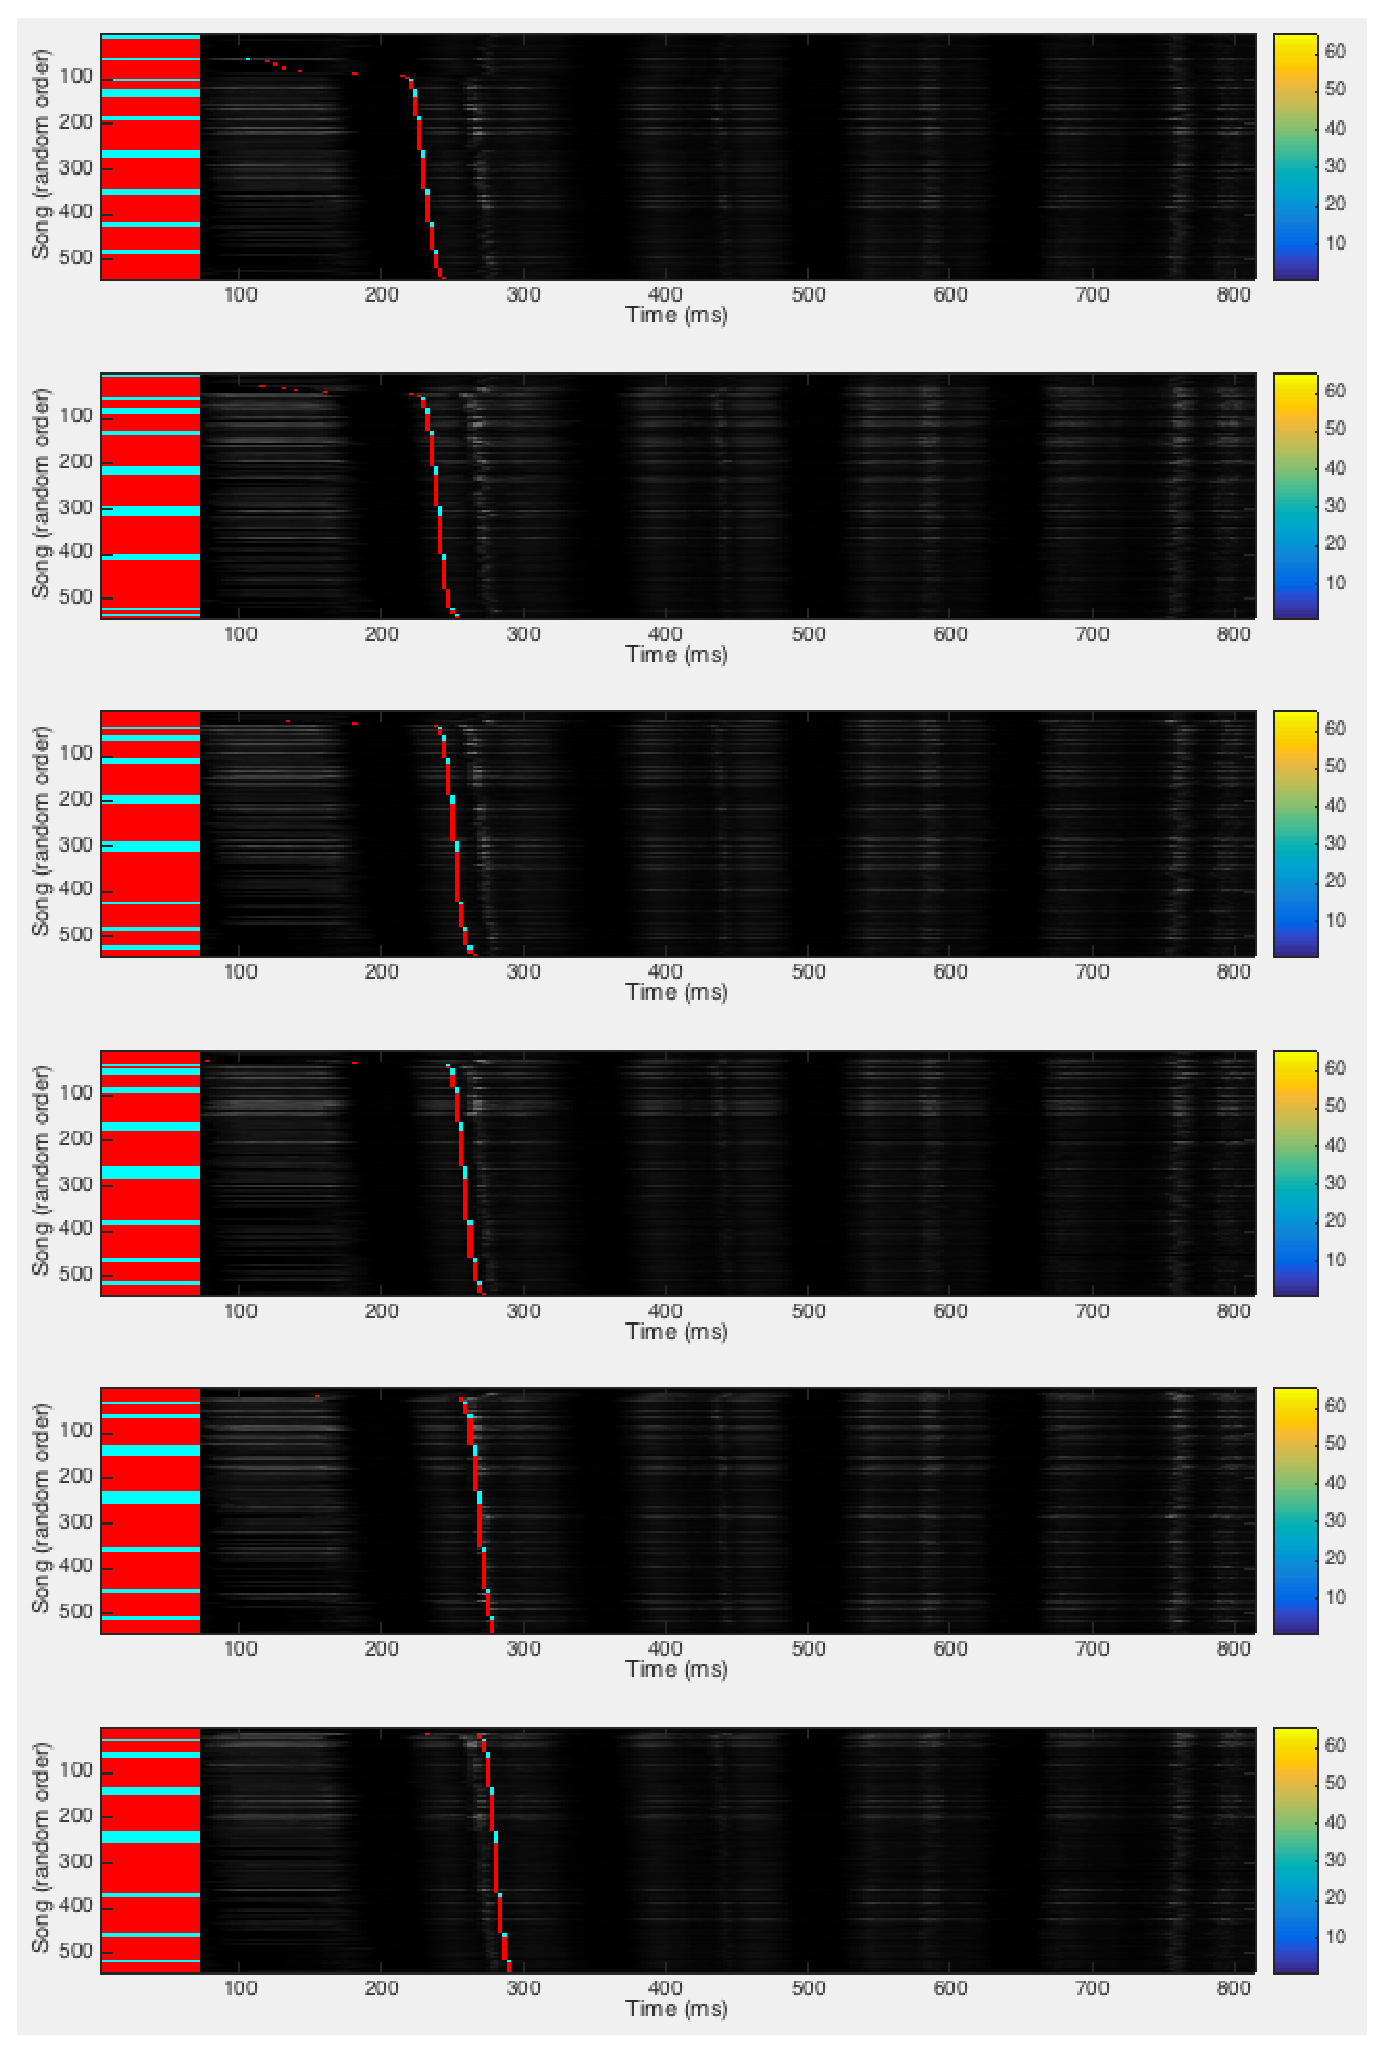
\includegraphics[width=\textwidth]{6_syllables_out}
    \caption{Detection results. Each plot shows detection events for
      the corresponding syllable as shown in
      \fig{fig:sixsyllables}. The horizontal axis is time, and the
      vertical axis is the index of the 526 single song
      presentations. The grey shading shows the total audio energy of
      song Y at time X. The bar on the left is the same width as the
      detection window, so no detection events can happen within that
      region, and its colour code shows training songs to the right of
      red regions and unseen test songs to the right of cyan
      regions. For visualisation of the distribution, songs have been
      stably sorted by the time of detection events.}
  \label{fig:sixsyllables_out}
\end{figure}

\begin{figure}
  \includegraphics[width=\textwidth]{6_syllables_roc}
  \caption{ROC curves for the detection of targets shown in Figure~\ref{fig:sixsyllables}. The first one, at the beginning of a syllable, is the most difficult to detect, and as more structure emerges in the current syllable, accuracy approaches 100\%.}
  \label{fig:roc}
\end{figure}

\begin{figure}
  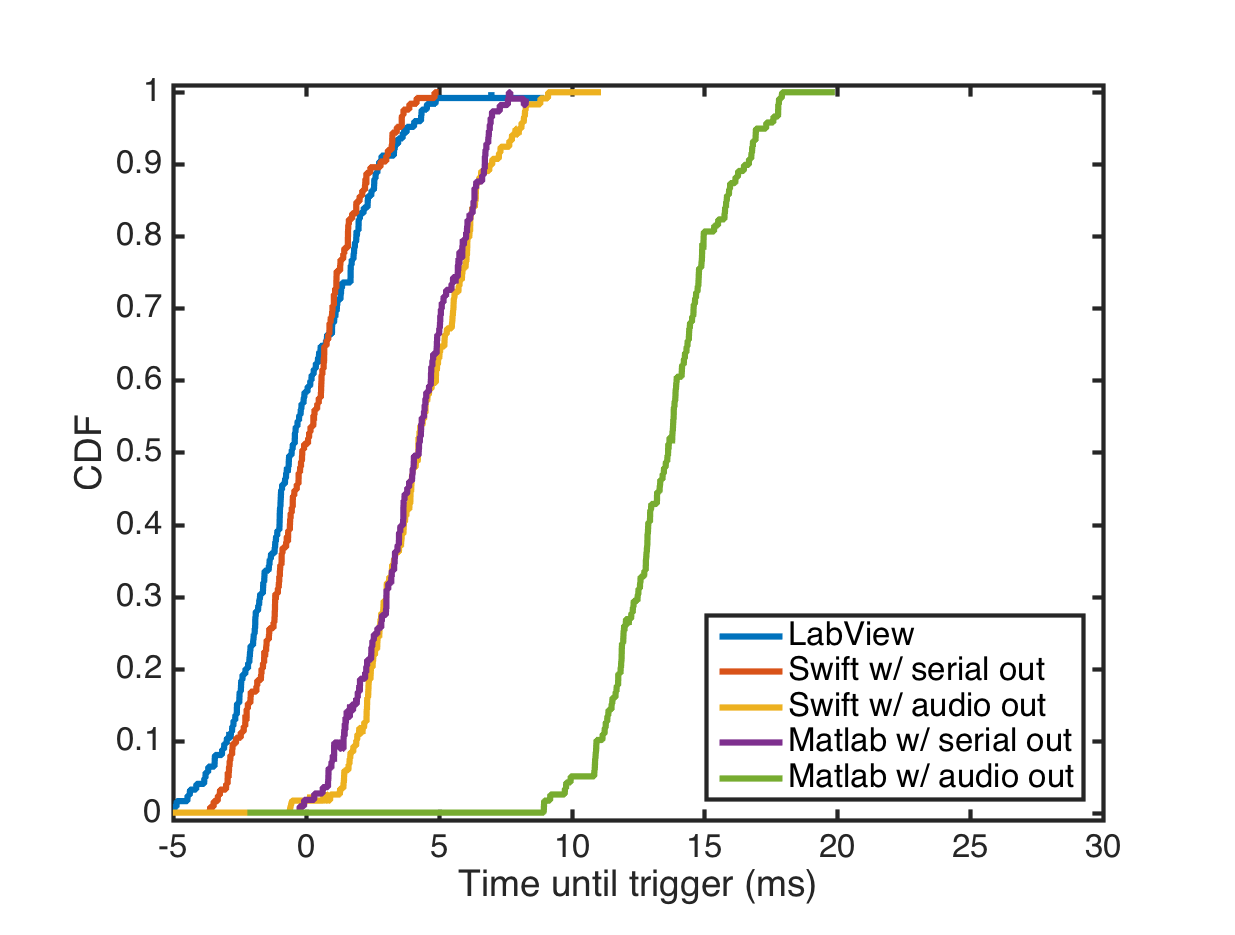
\includegraphics[width=\textwidth]{timing}
  \caption{Timing curve for a syllable running a test file generated by training.}
  \label{fig:timing}
\end{figure}


\section{Discussion}
\label{sec:conclusion}

This syllable detector is appropriate for zebra finch song, and although we did not test in other species, it is likely to work well for Bengalese finches and probably other species.  It offers the following benefits:
\begin{itemize}
\item The detector is accurate. False positive and false negative rates can both be well under 1\%, and trading these two numbers off against each other is through a single relative-cost parameter.
\item Latency can be around $3\pm1.2$ ms or better depending on hardware.
\item Works on a wide range of target syllables.
\item A single detector can easily generate different target pulses for multiple syllables, at almost no additional computational cost.
\item Requires no hand-tuning, although performance on certain syllables can be further improved if desired.
\item Runs in near realtime on inexpensive consumer-grade hardware, although we recommend that the training phase be run on a computer with at least 32GB of RAM.
\end{itemize}

As described, the detector only identifies matches that are similar to the training syllables.  A common experimental paradigm requires detecting the frequency of syllables.  Many pitch detection techniques rely on the spectrum, which is already available.  For example, \cite{Canopoli2014} achieved good results with the Harmonic Product Spectrum algorithm \cite{Noll1970}.

Duration detection is similarly easy.  The beginning and end of a syllable may be detected by looking at the ratio of total energy in the singing frequency band (approximately 1-7 kHz) to the total energy, over some small time window.  Any syllable thus identified that also contains a trigger event may be monitored for duration.  Alternatively, the network can be trained to recognise both the beginning and the end of the syllable of interest.

In feedback experiments such as frequency- or duration-shifting, vocal output changes over the course of the experiment.  The neural network excels at identifying syllables close to its training set, so as vocal output changes the detector may not recognise a match.  If the detector must be robust to this shift, it may be retrained every so often as the bird learns, or data consisting of synthetically pitch-shifted or duration-shifted target syllables over the recognition region may be added to the training set.  We will test these approaches in future work.

\section{Acknowledgments}
This work was funded by someone.\marginpar{But by whom?}

\appendix

\section{Resources}
\label{sec:resources}
\marginpar{PLOS doesn't really say where such things should go.}
\marginpar{Cleanup: mostly done.  But it would be nice to move all this to the lab's github group.}
\begin{description}
  \item[Song alignment:] Last we checked, Jeff Markowitz's song
    alignment software could be found at \\
    {\tt https://github.com/jmarkow}.

    \item[Training the neural network:] Our implementation of the syllable
      detector training code is available under the GNU GPL at:
      \\ {\tt https://github.com/bwpearre/}

    \item[Runtime:] The Matlab, Swift, and Labview implementations for executing the trained
      network:\\
      {\tt https://github.com/nathanntg/syllable-detector}
\end{description}

\bibliography{birds}

\end{document}

